\documentclass[margin=10pt]{standalone}
\usepackage{cmbright}
%\renewcommand{\familydefault}{\sfdefault}
%
\usepackage{tikz}
\usetikzlibrary{arrows}
\usetikzlibrary{arrows.meta}
\usetikzlibrary{backgrounds}
\usetikzlibrary{decorations.markings}
\usetikzlibrary{fit}
\usetikzlibrary{matrix}
\usetikzlibrary{positioning}
\usetikzlibrary{shadows}

\begin{document}
{
\normalsize
%\large

\newsavebox\mybox
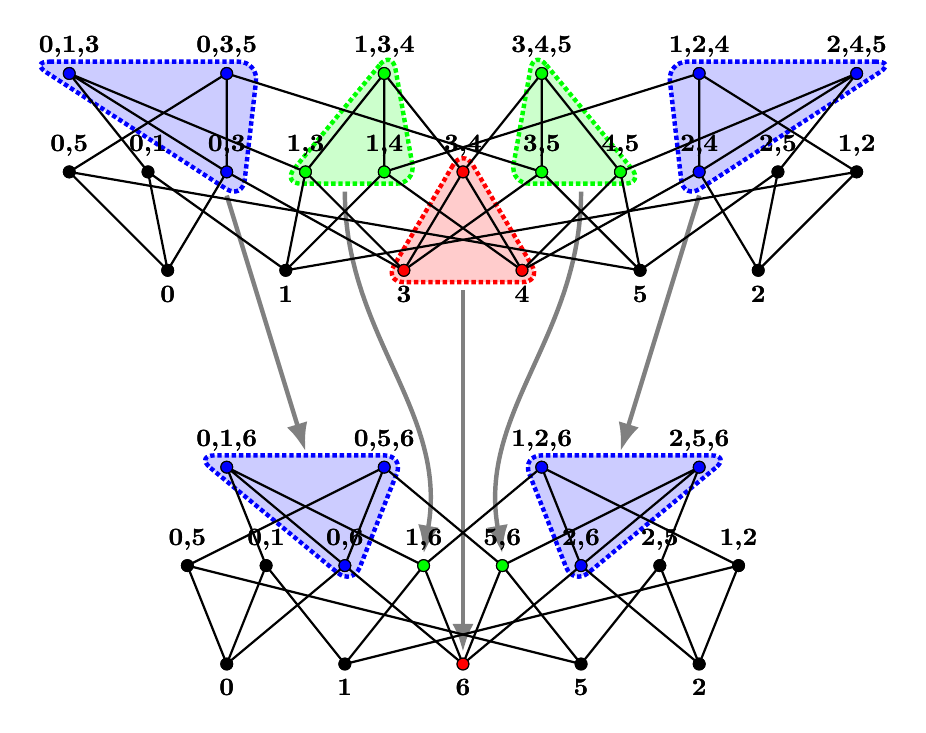
\begin{tikzpicture}[
		every node/.style = {
			draw,
			fill = white!5,
			align = center
		},
		every label/.style = {
			draw=none,
			fill=none,
			text=black, 
			font={\small\bfseries}
		},
		line/.style = {
			thick
		},
		point/.style = {
			fill=black,
			inner sep = 0pt,
			outer sep = 0pt,
			minimum size = 1.5mm, 
			circle
		},
		bgbox/.style = {
			ultra thick,
			densely dotted,
			rounded corners=0.25cm
		},
		arr/.style = {
			draw=gray,
			ultra thick,
        	-Latex
        },
 		]

	%\draw[step=1cm,black!80,very thin] (0,0) grid (15,8);
	%\draw[step=0.5cm,black!20,very thin] (0,0) grid (15,8);


%%%%%
% MAPPING ARROWS
%%%%%
	\draw[arr] (6cm,4.75cm) -- (6cm,0.15cm);
	\draw[arr] (4.5cm,6cm) to[out=-90, in=80] (5.5cm,1.4cm);
	\draw[arr] (7.5cm,6cm) to[out=-90, in=100] (6.5cm,1.4cm);
	\draw[arr] (3cm,5.95cm) to (4cm,2.7cm);
	\draw[arr] (9cm,5.95cm) to (8cm,2.7cm);


%%%%%%%%%%%%%%%%%%%%%%%%%%%%%%
% BEFORE ASC
%%%%%%%%%%%%%%%%%%%%%%%%%%%%%%
%% CIRCLE THINGS OF INTEREST
	\filldraw[draw=red, fill=red!20, bgbox] (6, 6.55) -- (5,4.85) -- (7,4.85) -- cycle;

	\filldraw[draw=green, fill=green!20, bgbox] (5.1, 7.8) -- (3.7,6.1) -- (5.4,6.1) -- cycle;
	\filldraw[draw=green, fill=green!20, bgbox] (6.9, 7.8) -- (8.3,6.1) -- (6.6,6.1) -- cycle;

	\filldraw[draw=blue, fill=blue!20, bgbox] (0.5,7.65) -- (3.4,7.65) -- (3.2,5.9) -- cycle;
	\filldraw[draw=blue, fill=blue!20, bgbox] (11.5,7.65) -- (8.6,7.65) -- (8.8,5.9) -- cycle;

%% ASC
	\pgfmathsetlengthmacro{\vb}{5cm};
	\pgfmathsetlengthmacro{\vo}{1.25cm};

	\pgfmathsetlengthmacro{\hb}{2.25cm};
	\pgfmathsetlengthmacro{\ho}{1.5cm};

	\coordinate[point,label={below:0}] (0) at (\hb,\vb);
	\coordinate[point,label={below:1}] (1) at (\hb+\ho,\vb);
	\coordinate[point,label={below:3}] (3) at (\hb+2*\ho,\vb);
	\coordinate[point,label={below:4}] (4) at (\hb+3*\ho,\vb);	
	\coordinate[point,label={below:5}] (5) at (\hb+4*\ho,\vb);
	\coordinate[point,label={below:2}] (2) at (\hb+5*\ho,\vb);


	\pgfmathsetlengthmacro{\vb}{\vb+\vo};
	\pgfmathsetlengthmacro{\hb}{1cm};
	\pgfmathsetlengthmacro{\ho}{1cm};

	\coordinate[point,label={0,5}] (05) at (\hb,\vb);
	\coordinate[point,label={0,1}] (01) at (\hb+\ho,\vb);
	\coordinate[point,label={0,3}] (03) at (\hb+2*\ho,\vb);
	\coordinate[point,label={1,3}] (13) at (\hb+3*\ho,\vb);
	\coordinate[point,label={1,4}] (14) at (\hb+4*\ho,\vb);
	\coordinate[point,label={3,4}] (34) at (\hb+5*\ho,\vb);
	\coordinate[point,label={3,5}] (35) at (\hb+6*\ho,\vb);
	\coordinate[point,label={4,5}] (45) at (\hb+7*\ho,\vb);
	\coordinate[point,label={2,4}] (24) at (\hb+8*\ho,\vb);
	\coordinate[point,label={2,5}] (25) at (\hb+9*\ho,\vb);
	\coordinate[point,label={1,2}] (12) at (\hb+10*\ho,\vb);

	\draw[line] (0) -- (01) -- (1);
	\draw[line] (0) -- (03) -- (3);
	\draw[line] (0) -- (05) -- (5);
	\draw[line] (1) -- (12) -- (2);
	\draw[line] (1) -- (13) -- (3);
	\draw[line] (1) -- (14) -- (4);
	\draw[line] (2) -- (24) -- (4);
	\draw[line] (2) -- (25) -- (5);
	\draw[line] (3) -- (34) -- (4);
	\draw[line] (3) -- (35) -- (5);
	\draw[line] (4) -- (45) -- (5);

	\pgfmathsetlengthmacro{\vb}{\vb+\vo};
	\pgfmathsetlengthmacro{\hb}{1cm};
	\pgfmathsetlengthmacro{\ho}{2cm};

	\coordinate[point,label={0,1,3}] (013) at (\hb,\vb);
	\coordinate[point,label={0,3,5}] (035) at (\hb+\ho,\vb);
	\coordinate[point,label={1,3,4}] (134) at (\hb+2*\ho,\vb);
	\coordinate[point,label={3,4,5}] (345) at (\hb+3*\ho,\vb);
	\coordinate[point,label={1,2,4}] (124) at (\hb+4*\ho,\vb);
	\coordinate[point,label={2,4,5}] (245) at (\hb+5*\ho,\vb);

	\draw[line] (01) -- (013) (03) -- (013) (13) -- (013);
	\draw[line] (03) -- (035) (05) -- (035) (35) -- (035);
	\draw[line] (13) -- (134) (14) -- (134) (34) -- (134);
	\draw[line] (12) -- (124) (14) -- (124) (24) -- (124);
	\draw[line] (24) -- (245) (25) -- (245) (45) -- (245);
	\draw[line] (34) -- (345) (35) -- (345) (45) -- (345);


%% REDUNDANT COORDS TO REDRAW LABELS
	\pgfmathsetlengthmacro{\vb}{5cm};

	\pgfmathsetlengthmacro{\hb}{2.25cm};
	\pgfmathsetlengthmacro{\ho}{1.5cm};

	\coordinate[point,label={below:0}] (0) at (\hb,\vb);
	\coordinate[point,label={below:1}] (1) at (\hb+\ho,\vb);
	\coordinate[point,label={below:3},fill=red] (3) at (\hb+2*\ho,\vb);
	\coordinate[point,label={below:4},fill=red] (4) at (\hb+3*\ho,\vb);	
	\coordinate[point,label={below:5}] (5) at (\hb+4*\ho,\vb);
	\coordinate[point,label={below:2}] (2) at (\hb+5*\ho,\vb);


	\pgfmathsetlengthmacro{\vb}{\vb+\vo};
	\pgfmathsetlengthmacro{\hb}{1cm};
	\pgfmathsetlengthmacro{\ho}{1cm};

	\coordinate[point,label={0,5}] (05) at (\hb,\vb);
	\coordinate[point,label={0,1}] (01) at (\hb+\ho,\vb);
	\coordinate[point,label={0,3},fill=blue] (03) at (\hb+2*\ho,\vb);
	\coordinate[point,label={1,3},fill=green] (13) at (\hb+3*\ho,\vb);
	\coordinate[point,label={1,4},fill=green] (14) at (\hb+4*\ho,\vb);
	\coordinate[point,label={3,4},fill=red] (34) at (\hb+5*\ho,\vb);
	\coordinate[point,label={3,5},fill=green] (35) at (\hb+6*\ho,\vb);
	\coordinate[point,label={4,5},fill=green] (45) at (\hb+7*\ho,\vb);
	\coordinate[point,label={2,4},fill=blue] (24) at (\hb+8*\ho,\vb);
	\coordinate[point,label={2,5}] (25) at (\hb+9*\ho,\vb);
	\coordinate[point,label={1,2}] (12) at (\hb+10*\ho,\vb);

	\pgfmathsetlengthmacro{\vb}{\vb+\vo};
	\pgfmathsetlengthmacro{\hb}{1cm};
	\pgfmathsetlengthmacro{\ho}{2cm};

	\coordinate[point,label={0,1,3},fill=blue] (013) at (\hb,\vb);
	\coordinate[point,label={0,3,5},fill=blue] (035) at (\hb+\ho,\vb);
	\coordinate[point,label={1,3,4},fill=green] (134) at (\hb+2*\ho,\vb);
	\coordinate[point,label={3,4,5},fill=green] (345) at (\hb+3*\ho,\vb);
	\coordinate[point,label={1,2,4},fill=blue] (124) at (\hb+4*\ho,\vb);
	\coordinate[point,label={2,4,5},fill=blue] (245) at (\hb+5*\ho,\vb);


%%%%%%%%%%%%%%%%%%%%%%%%%%%%%%
% AFTER ASC
%%%%%%%%%%%%%%%%%%%%%%%%%%%%%%
%% CIRCLE THINGS OF INTEREST
	\filldraw[draw=blue, fill=blue!20, bgbox] (2.6,2.65) -- (4.6,1) -- (5.25,2.65) -- cycle;
	\filldraw[draw=blue, fill=blue!20, bgbox] (9.4,2.65) -- (7.4,1) -- (6.75,2.65) -- cycle;

%% ASC
	\pgfmathsetlengthmacro{\vb}{0cm};
	\pgfmathsetlengthmacro{\hb}{3cm};
	\pgfmathsetlengthmacro{\ho}{1.5cm};

	\coordinate[point,label={below:0}] (0) at (\hb,\vb);
	\coordinate[point,label={below:1}] (1) at (\hb+\ho,\vb);
	\coordinate[point,label={below:6}] (6) at (\hb+2*\ho,\vb);
	\coordinate[point,label={below:5}] (5) at (\hb+3*\ho,\vb);
	\coordinate[point,label={below:2}] (2) at (\hb+4*\ho,\vb);


	\pgfmathsetlengthmacro{\vb}{\vb+\vo};
	\pgfmathsetlengthmacro{\hb}{2.5cm};
	\pgfmathsetlengthmacro{\ho}{1.0cm};

	\coordinate[point,label={0,5}] (05) at (\hb,\vb);
	\coordinate[point,label={0,1}] (01) at (\hb+\ho,\vb);
	\coordinate[point,label={0,6}] (06) at (\hb+2*\ho,\vb);
	\coordinate[point,label={1,6}] (16) at (\hb+3*\ho,\vb);
	\coordinate[point,label={5,6}] (56) at (\hb+4*\ho,\vb);
	\coordinate[point,label={2,6}] (26) at (\hb+5*\ho,\vb);
	\coordinate[point,label={2,5}] (25) at (\hb+6*\ho,\vb);
	\coordinate[point,label={1,2}] (12) at (\hb+7*\ho,\vb);

	\draw[line] (0) -- (01) -- (1);
	\draw[line] (0) -- (06) -- (6);
	\draw[line] (0) -- (05) -- (5);
	\draw[line] (1) -- (12) -- (2);
	\draw[line] (1) -- (16) -- (6);
	\draw[line] (2) -- (26) -- (6);
	\draw[line] (2) -- (25) -- (5);
	\draw[line] (6) -- (56) -- (5);

	\pgfmathsetlengthmacro{\vb}{\vb+\vo};
	\pgfmathsetlengthmacro{\hb}{3cm};
	\pgfmathsetlengthmacro{\ho}{2cm};

	\coordinate[point,label={0,1,6}] (016) at (\hb,\vb);
	\coordinate[point,label={0,5,6}] (056) at (\hb+\ho,\vb);
	\coordinate[point,label={1,2,6}] (126) at (\hb+2*\ho,\vb);
	\coordinate[point,label={2,5,6}] (256) at (\hb+3*\ho,\vb);

	\draw[line] (01) -- (016) (06) -- (016) (16) -- (016);
	\draw[line] (06) -- (056) (05) -- (056) (56) -- (056);
	\draw[line] (12) -- (126) (16) -- (126) (26) -- (126);
	\draw[line] (26) -- (256) (25) -- (256) (56) -- (256);



%% REDUNDANT CORODS TO REDRAW LABELS
	\pgfmathsetlengthmacro{\vb}{0cm};
	\pgfmathsetlengthmacro{\hb}{3cm};
	\pgfmathsetlengthmacro{\ho}{1.5cm};

	\coordinate[point,label={below:0}] (0) at (\hb,\vb);
	\coordinate[point,label={below:1}] (1) at (\hb+\ho,\vb);
	\coordinate[point,label={below:6}, fill=red] (6) at (\hb+2*\ho,\vb);
	\coordinate[point,label={below:5}] (5) at (\hb+3*\ho,\vb);
	\coordinate[point,label={below:2}] (2) at (\hb+4*\ho,\vb);

	\pgfmathsetlengthmacro{\vb}{\vb+\vo};
	\pgfmathsetlengthmacro{\hb}{2.5cm};
	\pgfmathsetlengthmacro{\ho}{1.0cm};

	\coordinate[point,label={0,5}] (05) at (\hb,\vb);
	\coordinate[point,label={0,1}] (01) at (\hb+\ho,\vb);
	\coordinate[point,label={0,6},fill=blue] (06) at (\hb+2*\ho,\vb);
	\coordinate[point,label={1,6},fill=green] (16) at (\hb+3*\ho,\vb);
	\coordinate[point,label={5,6},fill=green] (56) at (\hb+4*\ho,\vb);
	\coordinate[point,label={2,6},fill=blue] (26) at (\hb+5*\ho,\vb);
	\coordinate[point,label={2,5}] (25) at (\hb+6*\ho,\vb);
	\coordinate[point,label={1,2}] (12) at (\hb+7*\ho,\vb);

	\pgfmathsetlengthmacro{\vb}{\vb+\vo};
	\pgfmathsetlengthmacro{\hb}{3cm};
	\pgfmathsetlengthmacro{\ho}{2cm};

	\coordinate[point,label={0,1,6},fill=blue] (016) at (\hb,\vb);
	\coordinate[point,label={0,5,6},fill=blue] (056) at (\hb+\ho,\vb);
	\coordinate[point,label={1,2,6},fill=blue] (126) at (\hb+2*\ho,\vb);
	\coordinate[point,label={2,5,6},fill=blue] (256) at (\hb+3*\ho,\vb);

\end{tikzpicture}
}% end size


\end{document}   